% Appendix Template

\chapter{Registro de respuesta} % Main appendix title

\label{App_Estimulos} % Change X to a consecutive letter; for referencing this appendix elsewhere, use \ref{AppendixX}

\begin{figure}[th]
\centering
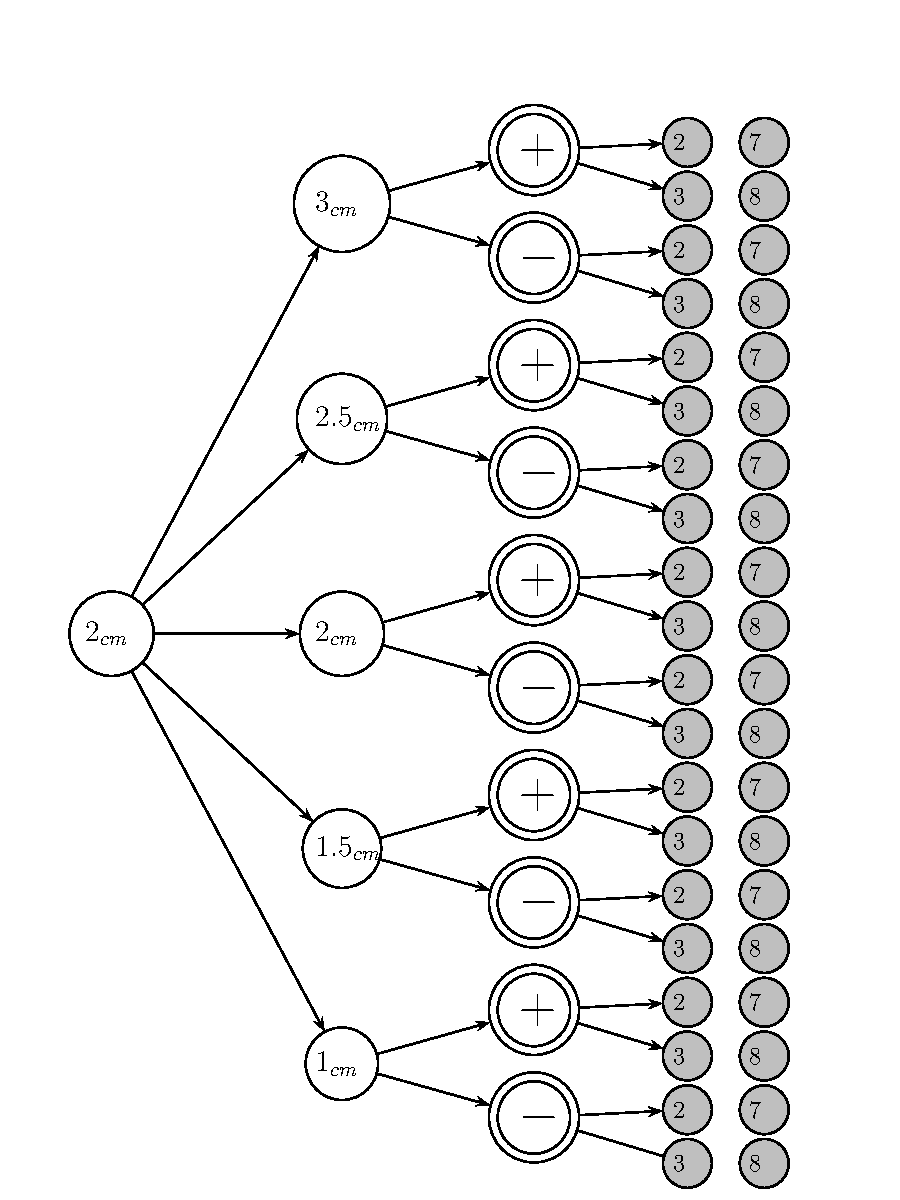
\includegraphics[width=0.99\textwidth]{Figures/Estimulos_Experimento1} 
\decoRule
\caption[Diseño de Estimulos en el Experimento 1]{Ilustración del diseño factorial 5x2x2 utilizado para construir las figuras de Ebbinghaus presentadas en el Experimento 1. En cada ensayo los participantes compararon el tamaño de un círculo de referencia constante (2cm de diámetro, ilustrado en el lado izquierdo de la figura) con el círculo central de una figura de Ebbinghaus que podía ser de cinco tamaños diferentes, con círculos externos que inducieran efectos de sobrestimación o subestimación (señalados con signos positivos y negativos, respectivamente) y con dos variaciones del 'número de círculos externo' dependientes de la condición (2 y 3 círculos externos en la condición fácil o 7 y 8 en la condición difícil). Por cada condición, se tienen 16 estímulos con ruido, (repetidos 10 veces cada uno en cinco colores diferentes) y cuatro que contienen la señal (presentados 40 veces cada uno, en cinco colores diferentes), dejándonos con 320 ensayos por condición y un total de 640 ensayos en todo el experimento.}
\label{fig:Exp_1}
\end{figure}

\begin{figure}[th]
\centering
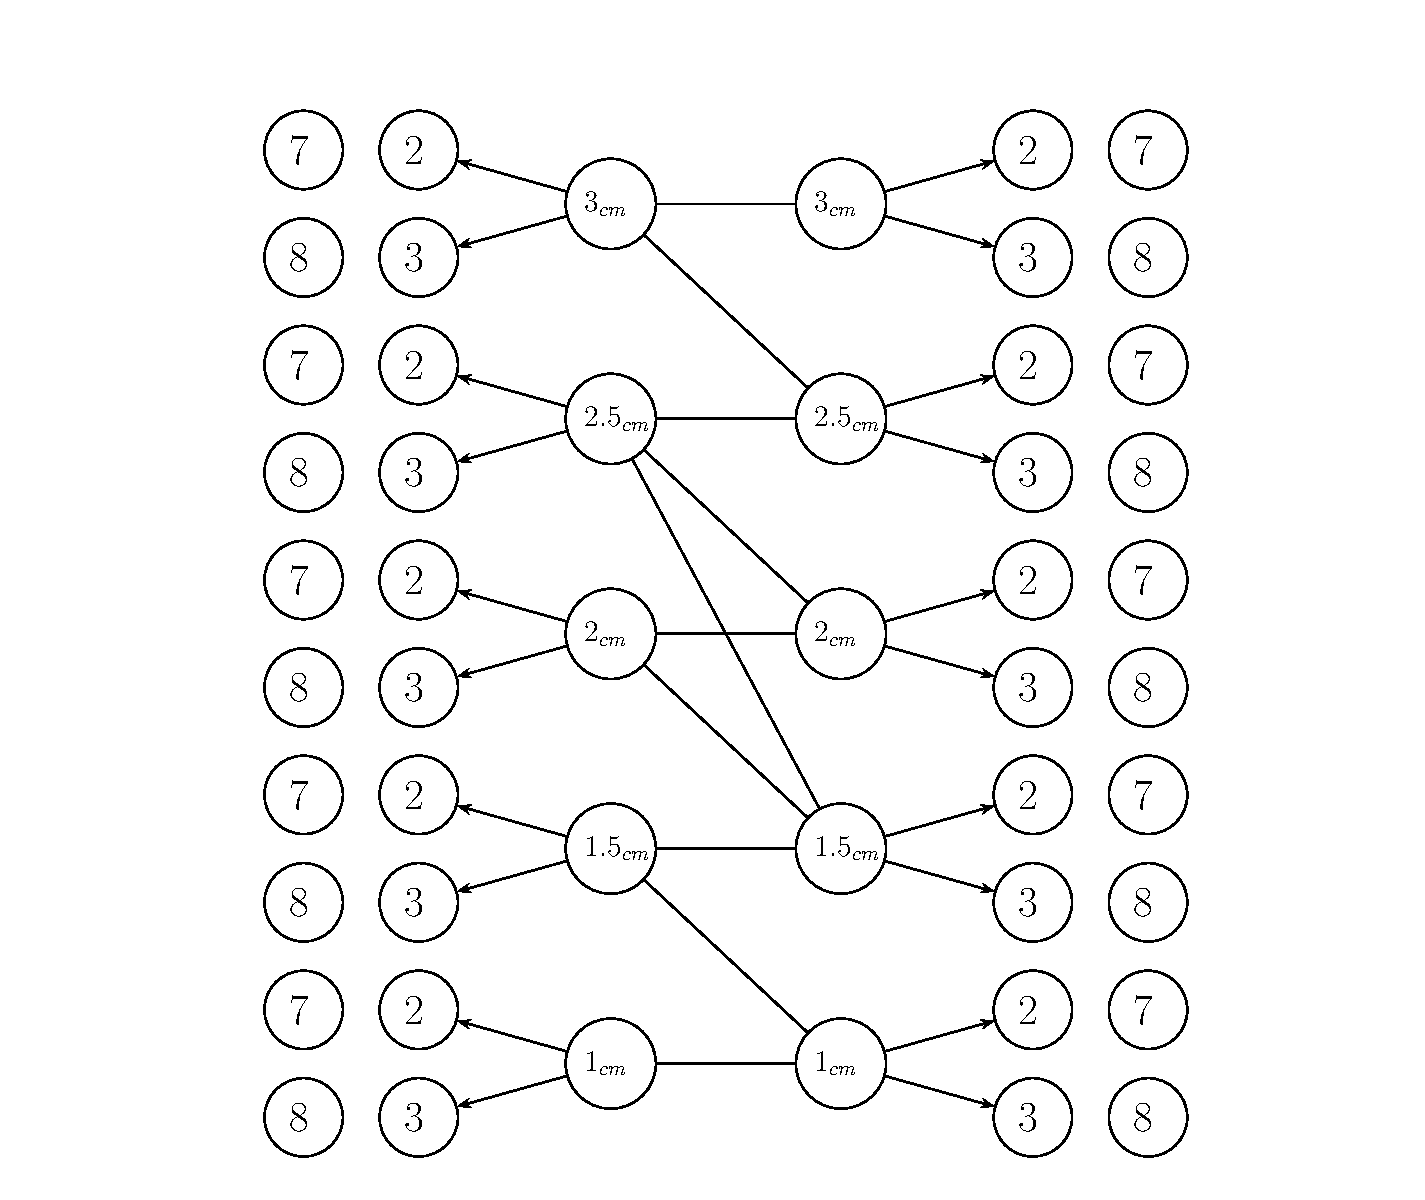
\includegraphics[width=0.9\textwidth]{Figures/Estimulos_Experimento2} 
\decoRule
\caption[Diseño de Estimulos en el Experimento 2]{Diseño de las parejas de figuras de Ebbinghaus mostradas en el Experimento 2, compuestas por una figura con efecto de subestimación y una con efecto de sobrestimación. Con los cinco tamaños distintos de círculo central propuestos se crearon cinco parejas iguales (señales) y cinco parejas arbitrarias desiguales (ruido). Por cada una de las diez parejas se consideró las cuatro combinaciones posibles entre los niveles de círculos externos incluídos en cada condición - 2 vs 2 o 7 vs 7; 3 vs 3 u 8 vs 8; 2 vs 3 o 7 vs 8; 3 vs 2 o 8 vs 7) Cada pareja se repitió ocho veces, contrabalanceando la posición derecha-izquierda de los efectos de sobrestimación y subestimación.}
\label{fig:Exp_2}
\end{figure}
\end{itemize}
